\chapter{Functions \& Maps}
\begin{chout}
	We now spend some time considering the different classes of functions and maps
	on Riemann surfaces. This will allow for extensive generalisations from the
	theory of complex analysis.
\end{chout}

\section{Holomorphic functions}
\begin{definition}[Holomorphicity]
	The complex-valued function $ f:X \to \mathbb{C} $ is said to be
	\defined{holomorphic at} $ x \in X $ if $ f \circ \phi ^{-1} $ is holomorphic at
	$ \phi(x) $ for every chart $ \phi: U \to \tilde{U} $ with $ x \in U $.

	$ f $ is \defined{holomorphic on} $ W \subseteq X $ if it is holomorphic at
	every point $ w \in W $.

	$ f $ is \defined{holomorphic} if it is holomorphic on $ X $.
\end{definition}

\begin{figure*}
	\centering
	\includegraphics{holomorphic-fct/figure}
	\caption{The function $ f $ is holomorphic (at/on) in line with the function $ f
			\circ \phi ^{-1} $.}
\end{figure*}

\begin{example}
	For a Riemann surface $ X $, with atlas $ \left\{ U _{\alpha}, \phi _{\alpha}
		\right\} $, the charts $ \phi _{\alpha}: U _{\alpha} \to \tilde{U} _{\alpha} $
	are holomorphic on $ U _{\alpha} $.
\end{example}

\begin{example}\label{ex:holo-C-algebra-1}
	Let $ f:X \to \mathbb{C}:x \to z_0 $ for $ z_0 \in \mathbb{C} $ constant. Since
	translative functions are holomorphic in the complex plane, the function $ f $
	is holomorphic at each point $ x \in X $, and hence holomorphic.
\end{example}

\begin{notation}
	It is common to denote the set of holomorphic functions on an open subset $ W
		\subseteq X $ of a Riemann surface $ X $ by $ \mathcal{O}(W) $.
\end{notation}

\begin{proposition}
	$ \mathcal{O}(W) $ is a $ \mathbb{C} $--algebra.
	\begin{proof}
		We recall that for this to be the case, we need that constant functions on $ W $
		are holomorphic, and that sums of holomorphic functions are holomorphic. Since
		the former was shown in Example~\ref{ex:holo-C-algebra-1} we proceed with the
		latter.

		Let $ f,g:W \to \mathbb{C} $ be holomorphic on $ W \subseteq X $, and let $ w
			\in W $. Considering a chart $ (U, \phi) $ at $ w $, and calling on the
		right-distributivity of function composition,
		\begin{align*}
			(f+g)\circ \phi ^{-1}(w) = (f \circ \phi ^{-1})(w) + (g \circ \phi ^{-1})(w)
		\end{align*}
		is a sum of functions which are holomorphic at $ \phi(w) $. The arbitrary
		choice of $ w $ ensures that $ f+g $ is indeed holomorphic on $ W $.
	\end{proof}
\end{proposition}

It is not at all surprising that with the basic definitions supplied, we can
find natural extensions of many results from complex
analysis\sidenote{\footnotesize\cite[p. 29]{miranda}}.

\begin{theorem}[Maximum modulus principle]\label{thm:max-mod}
	Let the function $ f:X \to \mathbb{C} $ be holomorphic on Riemann surface $ X $.
	If there exists a point $ x_0 \in X $ such that, $ |f(x)|\leq|f(x_0)| $ for all
	points $ x \in X $ then $ f $ is constant.
	\begin{proof}
		Suppose that the point $ x_0 $ exists, and consider the set $ \mathcal{X} =
			\left\{ x \in X: f(x)=f(x_0) \right\} $. We can alternatively formulate this set
		as the pre-image of the point $ f(x_0) $, i.e., $ \mathcal{X} = f ^{-1}(f(x_0))
		$, which is closed by the continuity of the function $ f $. Further to this, $
			\mathcal{X} $ is non-empty since $ x_0 \in \mathcal{X} $.

		Let $ \xi \in \mathcal{X} $, and let a chart about the point $ \xi $ be given by
		$ \phi:U \to \tilde{U} $. From the holomorphicity of $ f $ we know that the
		function $ f \circ \phi ^{-1} $ is holomorphic between open subsets of the
		complex plane. Additionally, we have that
		\begin{align*}
			|f(u)|\leq |f(\xi)| \quad \forall u \in U,
		\end{align*}
		which implies,
		\begin{align*}
			|(f \circ \phi ^{-1})(\phi(u))|\leq |(f \circ \phi ^{-1})(\phi(\xi))| \quad
			\forall u \in U.
		\end{align*}
		Then, by the maximum modulus principle (Theorem~\ref{thm:pre-max-mod}) the
		function $ f \circ \phi ^{-1} $ is constant on the connected open subset $
			\tilde{U} $. Consequently,
		\begin{align*}
			f(u) = (f \circ \phi ^{-1})(\phi(u)) = (f \circ \phi ^{-1})(\phi(\xi)) =
			f(\xi) = f(x_0)
		\end{align*}
		for all $ u \in U $, which determines that $ u \in \mathcal{X} $ for all $ u
			\in U $. This is equivalent to $ U \subseteq \mathcal{X} $, and the
		arbitrary choice of $ u $ gives the openness of $ \mathcal{X} $. Since $ X $ is
		connected $ \mathcal{X}=X $, and the statement is proved.
	\end{proof}
\end{theorem}

\begin{corollary}[Liouville]\label{cor:liouville}
	A holomorphic function $ f:X \to \mathbb{C} $ on a compact Riemann surface is
	constant.
	\begin{proof}
		We know that $ |f| $ is a continuous function since $ f $ is holomorphic, and
		the compactness of $ X $ assures that $ |f| $ attains its maximum at some point
		in $ X $. Theorem~\ref{thm:max-mod} determines that the function is constant,
		since $ X $ is connected.
	\end{proof}
\end{corollary}

\begin{example}
	Consider the torus examined in Section~\ref{sec:complex-tori}, $
		\mathbb{C}/\Lambda $, and the related projection map $ \pi:\mathbb{C} \to
		\mathbb{C}/\Lambda $. A function $ f:W \subseteq \mathbb{C}/\Lambda \to
		\mathbb{C} $ is holomorphic at a point $ w \in W $ if and only there exists a
	point $ z \in \pi ^{-1}(w) $ such that $ f \circ \pi $ is holomorphic at $ z $,
	a fact fairly easily observed by considering how we defined the complex charts
	on this space. Furthermore, $ f $ is holomorphic on $ W $ if and only if $ f
		\circ \pi $ is holomorphic on the pre-image of this subset, $ \pi ^{-1}(W) $.

	We now consider the case where $ W = \mathbb{C}/\Lambda $ referring to
	Varolin\sidenotemark. Considering an entire function $ f ^{*} $ we aim to
	determine the necessary criteria such that there exists a function $ f $, as
	above, with $ f ^{*} = f \circ \pi $. In order for this to be the case,
	we need $ f ^{*} $ to be invariant under the action of the lattice $ \Lambda
	$. In other words, we need $ f ^{*}(z) = f ^{*}(z + \lambda) $ for all $
		\lambda \in \Lambda $. Functions with this property are referred to as doubly
	periodic, and by the constancy of $ f $ as a holomorphic function on a compact
	Riemann surface, these functions are constant also.
\end{example}
\sidenotetext[][-9\baselineskip]{\footnotesize\cite{varolin}}

Corollary~\ref{cor:liouville} is perhaps indicative that there is less to
explore in the realm of holomorphic functions on Riemann surfaces, than there
was in the complex plane. Generalisation of another class of functions from
complex analysis proves more fruitful.

\section{Meromorphic functions}\label{sec:mero-fcts}
\begin{definition}[Meromorphicity]
	The complex-valued function $ f:X \to \mathbb{C} $ is said to be
	\defined{meromorphic at} $ x \in X $ if $ f \circ \phi ^{-1} $ is meromorphic
	at $ \phi(x) $, for every chart $ \phi:U \to \tilde{U} $ with $ x \in U $.

	$ f $ is \defined{meromorphic on} $ W \subseteq X $ if it is meromorphic at
	every point $ w \in W $.

	$ f $ is \defined{meromorphic} if it is meromorphic on $ X $.
\end{definition}

\begin{notation}
	It is common to denote the set of meromorphic functions on an open subset $ W
		\subseteq X $ of a Riemann surface $ X $ by $ \mathcal{M}(W) $.
\end{notation}

\begin{example}
	From our definition it is clear that every holomorphic function is meromorphic,
	and hence, for an open subset $ W \subseteq X $, $ \mathcal{O}(W) \subseteq
		\mathcal{M}(W) $.
\end{example}

\begin{example}
	Rational functions on $ \hat{\mathbb{C}} $ are meromorphic.

	We recall that rational functions are those which can be expressed as the
	quotient of polynomials, with denominator not identically $ 0 $. Denoting the
	ring of polynomials functions over $ \mathbb{C} $ by $ \mathbb{C}[z] $, any
	rational function $ f: \hat{\mathbb{C}} \to \mathbb{C} $ can be expressed as
	\begin{align*}
		f(z) = \frac{p(z)}{q(z)},
	\end{align*}
	where $ p \in \mathbb{C}[z] $ and $ q \in \mathbb{C}[z]\setminus \left\{ 0
		\right\} $. The algebraic closedness of $ \mathbb{C} $ determines that both $ p
	$ and $ q $ are entirely factorable;
	\begin{align*}
		\frac{p(z)}{q(z)} = \frac{(z-z _{p_1})\cdots(z-z _{p_m})}{(z-z
		_{q_1})\cdots(z-z _{q_n})},
	\end{align*}
	and hence the function has poles at the points $ z _{q_i} $, while being
	holomorphic away from these points, with some nuance related to cancellation
	of factors.
\end{example}

We can again generalise some well-known results from complex analysis.

\begin{theorem}[Principle of Isolation]
	The zeroes and poles of a meromorphic function $ f:X \to \mathbb{C} $ which is
	not identically zero form a discrete subset of $ X $.
	\begin{proof}
		Suppose that this wasn't the case, and let $ \left\{ x_i \right\} $ be a
		sequence of roots of $ f $ in $ X $ with a limit point $ x \in X $. Then $
			f(x)=0 $ and this is a limit point of the sequence $ \left\{ f(x_i) \right\}
		$ in $ \mathbb{C} $. By the Identity theorem, the function $ f $ must be
		identically $ 0 $. A similar argument for the function $ 1/f $ gives proof
		for the case of the poles.
	\end{proof}
\end{theorem}

\begin{corollary}\label{cor:finite-poles}
	A meromorphic function $ f:X \to \mathbb{C} $ on a compact Riemann surface $ X $
	which is not identically zero has a finite number of zeros and poles.
\end{corollary}

\begin{example}\label{ex:mero-rational-Ch}
	Meromorphic functions on $ \hat{\mathbb{C}} $ are rational.

	Let $ f:\hat{\mathbb{C}} \to \mathbb{C} $ be a meromorphic function.
	Corollary~\ref{cor:finite-poles} allows us to enumerate the zeroes and poles of
	this function. Let there be $ n $ zeroes, with orders $ e_{i} $, and $ m $
	poles with orders $ f_{j} $. If $ m=0 $, $ f $ is holomorphic and hence
	constant by the compactness of $ \hat{\mathbb{C}} $.

	We assume that $ n\geq 1 $ and construct the function
	\begin{align*}
		g(z) = f(z)\cdot \frac{\prod_{i=1}^{n}{(z-z_i)
		^{e_i}}}{\prod_{j=1}^{m}{(z-z_j)^{f_j}}},
	\end{align*}
	which is a meromorphic function of the Riemann sphere without zeroes or poles in
	the complex plane. It must be the case that either $ g $ or $ 1/g $ is
	holomorphic at $ z=\infty $ and hence the $ g(z) = c \in \mathbb{C} $, which
	via algebraic manipulation gives
	\begin{align*}
		f(z) = c\cdot \frac{\prod_{i=1}^{n}{(z-z_i)
		^{e_i}}}{\prod_{j=1}^{m}{(z-z_j)^{f_j}}},
	\end{align*}
	and $ f $ is rational.
\end{example}

The Laurent series of a meromorphic function is an important construction in
complex analysis, and turns out to also be important for meromorphic functions
on Riemann surfaces. If we have a function $ f:X \to \mathbb{C} $ which is
meromorphic at a point $ x \in X $, we can expand the corresponding locally read
meromorphic function $ f \circ \phi ^{-1} $, as a Laurent series. It is
important to note that contrary to the concepts which we have thus far
encountered, the Laurent series of $ f \circ \phi ^{-1} $ \textit{is} dependent
on the choice of chart.

\begin{definition}[Order]
	Let $ f:X \to \mathbb{C} $ be meromorphic at $ x \in X $. The \defined{order}
	of $ f $ at $ x $ is
	\begin{align*}
		\ord(f;x) = \min \left\{ n : c_n \neq 0 \right\},
	\end{align*}
	where $ c_i $ are the coefficients of the local Laurent series of $ f $, i.e.,
	$ f \circ \phi_{x}^{-1} $.
\end{definition}

Initially, the notion of order maybe seems more contrived than it does useful.
It will however have great importance as we reach the latter stages of our
progression, in particular in Chapter~\ref{ch:riemann-roch}. To continue our
exposition of the meromorphic functions on the Riemann sphere, we consider the
following example\sidenote{\footnotesize\cite[p. 27]{miranda}}, which will
undergo generalisation later.

\begin{example}
	A meromorphic function $ f: \hat{\mathbb{C}} \to \mathbb{C} $ is such that
	\begin{align*}
		\sum_{z \in \hat{\mathbb{C}}}^{}{\ord(f;z)}=0.
	\end{align*}

	We know from Example~\ref{ex:mero-rational-Ch} that all meromorphic functions
	can be expressed rationally, and complete factorisation of this rational
	expression gives us that
	\begin{align*}
		f(z) = c \cdot
		\frac{\prod_{i=1}^{n}{(z-z_i)^{e_i}}}{\prod_{j=1}^{m}{(z-z_j)^{f_j}}},
	\end{align*}
	where $ e_i, f_j \in \mathbb{N} $, and $ c \in \mathbb{C}\setminus \left\{ 0
		\right\} $. Alternatively, letting indices range over the integers gives us
	the expression,
	\begin{align*}
		f(z) = c \cdot \prod_{k}^{}{(z-z_k) ^{\alpha_k}.}
	\end{align*}
	We observe that $ \ord(f;z_k) = \alpha_k $, and away from these points the
	only non-zero order is found at $ z= \infty $. In particular, the order at
	this point is given by $ \ord(f; \infty) = \sum_{i}^{}{e_i}- \sum_{j}^{}{f_j}=
		-\sum_{k}^{}{\alpha_k}$. Then,
	\begin{align*}
		\sum_{z \in \hat{\mathbb{C}}}^{}{\ord(f;z)} = \sum_{i}^{}{\alpha_i}-
		\sum_{i}^{}{\alpha_i}=0.
	\end{align*}
\end{example}

\section{Holomorphic maps}
Category theory tells us that a natural next step in our study is the
consideration of maps between our objects of interest. In many ways, the
remaining sections in the chapter provide generalisation of those already seen.
Let $ X $ and $ Y $ be Riemann surfaces with atlases $ \left\{ U, \phi \right\}
$ and $ \left\{ V, \psi \right\} $ respectively.

\begin{definition}[Holomorphicity]\label{def:holomorphic}
	The map $ F:X \to Y $ is said to be \defined{holomorphic at} $ x \in X $ if, for
	all charts $ \phi:U \to \tilde{U} $ with $ x \in U $ and $ \psi: V \to \tilde{V}
	$ with $ F(x) \in V $, the composition
	\begin{align*}
		\psi \circ F \circ \phi ^{-1}: \phi(U \cap V) \to \psi(U \cap V) \\
	\end{align*}
	is holomorphic at $ \phi(x) $.

	$ F $ is \defined{holomorphic on} $ W \subseteq X $ if it is holomorphic at
	every point $ w \in W $.

	$ F $ is \defined{holomorphic} if it is holomorphic on $ X $.
\end{definition}

\begin{figure*}
	\centering
	\includegraphics{rs-maps/figure}
	\caption{The map $ F $ is holomorphic if and only if the map $ f $ is
		holomorphic.}
	\label{fig:rs-maps}
\end{figure*}

\begin{remark}
	We have seen that $ \mathbb{C} $ is a non-compact Riemann surface, and hence a
	holomorphic function is simply a holomorphic map to the complex plane.

	It is also worth noting the convention seen in Figure~\ref{fig:rs-maps}. We
	tend to refer to maps specifically between Riemann surfaces by capital
	letters, e.g., $ F $, and the corresponding local representation of the map by
	the corresponding lower case letter, e.g., $ f $.
\end{remark}

\begin{example}\label{ex:holo-id}
	The most basic example is that of the identity map $ \mathrm{id}:X \to X:x
		\mapsto x $. This map is easily seen to be holomorphic since, for any charts $
		\phi_i $ and $ \phi_j $ defined on a neighbourhood of the point $ x $ we have
	that
	\begin{align*}
		\phi_i \circ \mathrm{id} \circ \phi_j ^{-1} & = \phi_i \circ \phi_j ^{-1} \\
		                                            & = \phi _{i,j}
	\end{align*}
	is a transition function, and hence definitively holomorphic.
\end{example}

The fact that identity functions are holomorphic in this
framework allows us to make a further statement, of category theoretic
flavour\sidenote{\footnotesize\cite[p. 39]{miranda}}.

\begin{proposition}
	Riemann surfaces, and the holomorphic maps between them, form a category.
	\begin{proof}
		Example~\ref{ex:holo-id} showed the identity map to be holomorphic, and hence it
		remains to show that the composition of holomorphic maps is holomorphic. Let $
			F:X \to Y $ and $ G:Y \to Z $ be holomorphic maps between Riemann surfaces, $
			X,Y,Z $ with atlases $ \left\{ U, \phi \right\}, \left\{ V, \psi \right\},
			\left\{ W, \sigma \right\} $ respectively.

		Consider a point $ x \in X $, and let $ f = \psi \circ F \circ \phi ^{-1} $
		which is holomorphic at $ \phi(x) $. Let $ y = F(x) $, and let $ g = \sigma
			\circ G \circ \psi ^{-1} $ which is holomorphic at $ \psi(y) $. The composition
		\begin{align*}
			g \circ f & = \left(\sigma \circ G \circ \psi ^{-1}\right)\circ \left( \psi
			\circ F \circ \phi ^{-1} \right)                                            \\
			          & = \sigma \circ G \circ F \circ \phi ^{-1}
		\end{align*}
		is holomorphic at $ \phi(x) $, and the arbitrary choice of $ x $ means that $ G
			\circ F$ is holomorphic.
	\end{proof}
\end{proposition}

Tying the loose ends which we left at the end of
Chapter~\ref{ch:manifold-theory}, we can consider Riemann surfaces to be
equivalent if there exists a bijective holomorphic map with holomorphic inverse
between them\sidenote{\footnotesize\cite[p. 10]{donaldson}}. In this case, we
say that the Riemann surfaces are \defined{biholomorphic}.

\begin{remark}
	An earlier remark made mention of the fact that holomorphic functions are
	nothing more than a specification of holomorphic maps, made by choosing the
	codomain to be $ \mathbb{C} $. A very similar remark can be made for
	meromorphic functions and the Riemann sphere, $ \hat{\mathbb{C}} $.

	Let $ f:X \to \mathbb{C} $ be a meromorphic function, and define a map $ F:X \to
		\hat{\mathbb{C}} $ such that
	\begin{align*}
		F(x) = \begin{cases}
			       f(x)   & \text{if $ x $ is not a pole of $ f $}, \\
			       \infty & \text{if $ x $ is a pole of $ f $}.
		       \end{cases}
	\end{align*}
	This function is holomorphic away from the poles of $ f $ since $ f $ is
	definitively as such. Furthermore, $ F $ is holomorphic at the poles of $ f $
	and thus holomorphic.
\end{remark}

\section{The local model}
It is interesting to note that in our definition of holomorphicity we required
that the local representation of the map was holomorphic with respect to
\textit{every} pair of charts. There is a natural question which arises from
this: are there charts in which the local form is more `nicely' represented than
others? This is indeed the case, and in fact we can make a guarantee on the form
of these local charts in their `nicest' form. Before stating this, we consider
two lemmas which give a complete local description of holomorphic maps on
Riemann surfaces\sidenote{\footnotesize\cite[p. 43]{donaldson}}. Let $ f:U \to
	\mathbb{C} $ be a holomorphic function defined on an open neighbourhood $ U $ of
$ 0 \in \mathbb{C} $, such that $ f(0)=0 $.

\begin{lemma}\label{lem:local-model-1}
	If $ f'(0) \neq 0 $, there exists a neighbourhood $ U' \subset U $ of $ 0 $
	such that $ U' $ is homeomorphic to its image under $ f $, and $ f $ has
	holomorphic inverse on $ U' $.
\end{lemma}

\begin{lemma}\label{lem:local-model-2}
	If $ f \not \equiv 0 $, there exists a unique integer $ m \geq 1 $ and a
	holomorphic function $ g:U' \to \mathbb{C} $ defined on some neighbourhood $
		U' \subset U $ of $ 0 $ such that $ f(z) = g(z)^{m} $ on $ U' $ and $
		g'(0)\neq0 $.
\end{lemma}

\begin{theorem}[Local Normal Form]\label{thm:local-normal-form}
	Let $ F:X \to Y $ be a non-constant holomorphic map between Riemann
	surfaces $ X $ and $ Y $. For any $ x \in X $ there are charts around $ x $,
	and $ F(x)\in Y$ such that the local expression of $ F $ under these charts is
	given by $ z \mapsto z^m $ for some unique integer $ m\geq 1 $.
	\begin{proof}
		Suppose we have a holomorphic map $ F $ as described, and consider the local
		representation of this map in arbitrary charts about a point $ x \in X $ and
		the point $ F(x) \in Y $. We denote this local representation by $ f = \psi
			\circ F \circ \phi ^{-1} $, and apply Lemma~\ref{lem:local-model-2} to find
		a function $ g $ defined on a smaller domain such that $ f = g^m $. We know
		that ther derivative of $ g $ is non-vanishing at $ 0 $, and we can hence
		state, with reference to Lemma~\ref{lem:local-model-1}, that $ g $ is a
		biholomorphism. We can therefore compose $ g $ with the arbitrary charts we
		started with to find charts which have the desired property.
	\end{proof}
\end{theorem}

\begin{marginfigure}[-15\baselineskip]
	\centering
	\includegraphics{inverse-fct-thm/figure}
	\caption{Lemma~\ref{lem:local-model-1} is an inverse function theorem type
		statement.}
\end{marginfigure}

We now have a full understanding of the possible holomorphic maps between
Riemann surfaces locally, and the aim of globalising this idea is a natural next
step. Before completing this process, we state yet another generalisation from
complex analysis.

\begin{corollary}[Open Mapping Theorem]
	A non-constant holomorphic map $ F:X \to Y $ is open.
\end{corollary}

\section{Multiplicity and Degree}
In order to globalise this local model of holomorphic maps, we must restrict our
consideration to compact Riemann surfaces.

\begin{definition}[Multiplicity]
	The \defined{multiplicity} of a point $ x \in X $ under a map $ F:X \to Y $ is
	the unique integer $ m $ such that there is a local representation of the map
	as $ z \mapsto z^m $. We denote this by $ \mult(F;x) $.
\end{definition}

\begin{figure*}
	\centering
	\includegraphics{z^n-degree/figure}
	\caption{The only ramification point is at $ z=0 $.}
	\label{fig:z^n-degree}
\end{figure*}

If $ \mult(F;x) > 1 $, we call $ x $ a \defined{ramification point}, and the
image of a ramification point, is called a \defined{branch point}. Intuition for
these concepts is not hard to come by; consider the entire map $ f:z \mapsto z^3
$, for example. The following explanation will be best understood with relation
to Figure~\ref{fig:z^n-degree}.

In neighbourhoods of each of the points $ z_i \in \mathbb{C}^{*} $, $ z_i $ is
the only point such that $ f(z_i) = \omega $, and so locally, we can represent
this map as constant, and in particular we have that $ \mult(f;z_{i}) = 1 $. Now
consider the point $ 0 \in \mathbb{C} $, and furthermore a neighbourhood $ U $
of $ 0 $. For every point $ u \in U \setminus \left\{ 0 \right\}$ there are two
other points which all, under $ f $, map to the same point. Hence the local
normal form at $ 0 $ is exactly $ z \mapsto z^3 $, and $ \mult(f;0)=3 $. From
this we can see that $ 0 $ is the only ramification point of the map $ f $.

\begin{remark}
	This is a basic, but important example, especially since
	Theorem~\ref{thm:local-normal-form} told us that any map $ F:X \to Y $ can be
	read locally in this way.
\end{remark}

\begin{definition}[Degree]
	The \defined{degree} of a point $ y \in Y $ under a map $ F:X \to Y $ is the
	sum of the multiplicities of points in the pre-image of $ y $. Notatively,
	\begin{align*}
		\deg(F;y) = \sum_{x \in F ^{-1}(y)}^{}{\mult(F;x)}.
	\end{align*}
\end{definition}

\begin{figure*}
	\centering
	\includegraphics{local-normal-deg-mult/figure}
	\caption{We have that $ \mult(F;x_i)=m_i $ and that $ \deg(F;y)=m_1+m_2 $.}
\end{figure*}

Referring back to the example of $ f:z \mapsto z^3 $, we note that the degree of
the map is constant, since $ \deg(F;\omega)=3 $ for all $ \omega \in \mathbb{C}
$. We can follow a similar line of argument to show the constancy of the degree
under a map $ g:z \mapsto z^n $ for $ n \geq 1 $, and it is natural to question
whether this is a general phenomenon, for all holomorphic maps. This is indeed
the case, as summarised in the following proposition.

\begin{proposition}\label{prop:constant-degree}
	For a non-constant holomorphic map $ F:X \to Y $ between compact Riemann
	surfaces $ X $ and $ Y $, the degree $ \deg(F;y) $ is constant over all $ y \in
		Y$.
\end{proposition}

\begin{notation}
	Motivated by this result, we alter our notation, and refer to the degree of a
	map $ F:X \to Y $ by $ \deg(F) $, removing the dependence on the point in the
	codomain.
\end{notation}

To finish the chapter, we find a relation between the degree of a holomorphic
map between compact Riemann surfaces, and their respective genera. The result is
the Riemann--Hurwitz formula, stated by Riemann, and later proved by Adolf
Hurwitz\sidenote{\footnotesize\cite{hurwitz}}. There are a number of different
proofs of this result, in flavours topological\sidenote{\footnotesize\cite[p.
		100]{donaldson}}, algebraic\sidenote{\footnotesize\cite[p. 90]{griffiths}}, and
analytic\sidenote{\footnotesize\cite[p. 140]{forster}}.

\begin{theorem}[Riemann--Hurwitz Formula]
	Let $ F:X \to Y $ be a non-constant holomorphic map between compact Riemann
	surfaces. Then,
	\begin{align*}
		2 g(X) - 2 = \deg(F) (2 g(Y) - 2) + \sum_{x \in X}^{}{[\mult(F;x)-1]}.
	\end{align*}
\end{theorem}

\begin{example}
	Let $ F(x,y,z)=x^d+y^d+z^d $ and let $ X $ be the associated zero locus in
	projective space. Explicitly,
	\begin{align*}
		X = \left\{ [x:y:z]\in \mathbb{C}\mathbb{P}^{2}: F(x,y,z)=0 \right\}.
	\end{align*}
	We know from Section~\ref{sec:projective-curves}, the homogeneity and
	non-singularity of $ F $ determine that $ X $ is a compact Riemann surface,
	and we aim to compute the genus of this Riemann surface. With $ \pi $ as a
	projection map defined by
	\begin{align*}
		\pi:X \to \mathbb{C}\mathbb{P}^{1}:[x:y:z] \mapsto [x:y],
	\end{align*}
	we call on the fact\sidenotemark\ that a point $ p \in X $ is a ramification
	point under $ \pi $ if and only if $ \partial F/\partial z=0 $. If we
	take $ \alpha = [1:0] \in \mathbb{C}\mathbb{P}^{1} $ it cannot be the case that
	this is a branch point since $ z \neq 0 $ in order that $ \pi ^{-1}( \alpha)
		\subseteq X $. We must have that $ 1+z^d=0 $, and this occurs only at the $ d
	$ roots of unity, all of which are non-zero. Therefore,
	\begin{align*}
		\deg(\pi) = d.
	\end{align*}

	Proposition~\ref{prop:constant-degree} tells us that this is the degree of any
	point in $ \mathbb{C}\mathbb{P}^{1} $. To proceed we consider the point $
		\beta = [1:y] \in \mathbb{C}\mathbb{P}^{1} $ such that $ 1+y^d=0 $. For points
	of this form, it must be the case that pre-images have $ z=0 $, and in
	particular, that $ |\pi ^{-1}(\beta)|=1 $. There are $ d $ solutions to the
	equation $ 1+y^d=0 $, and since every point in $ \mathbb{C}\mathbb{P}^{1} $ can be
	represented in the form $ [1:\gamma] $ for some $ \gamma \in \mathbb{C} $, we
	see that these $ d $ solutions are the only possible branch points in the
	codomain. Applying (and rearranging) the formula, we find that
	\begin{align*}
		g ( X ) = \frac{( d-1 )( d-2 )}{2}.
	\end{align*}
\end{example}
